%%%%%%%%%%%%%%%%%%%%%%%%%%%%%%%%%%%%%%%%%%%%%%%%%%%%%%%%%%%%%%%%%%%%%%%%%%%%%%%%%%%%%%%%%%%%%%%%%%%%%%%%%%%%%%%%%%%%%%%%%%%%%%%%%%%%%%%%%%%%%%%%%%%%%%%%%%%%%%%%%%%%%%%%%%%%%%

\UC{Checkout}
\label{checkout}

\begin{figure}[H]
    \centering
    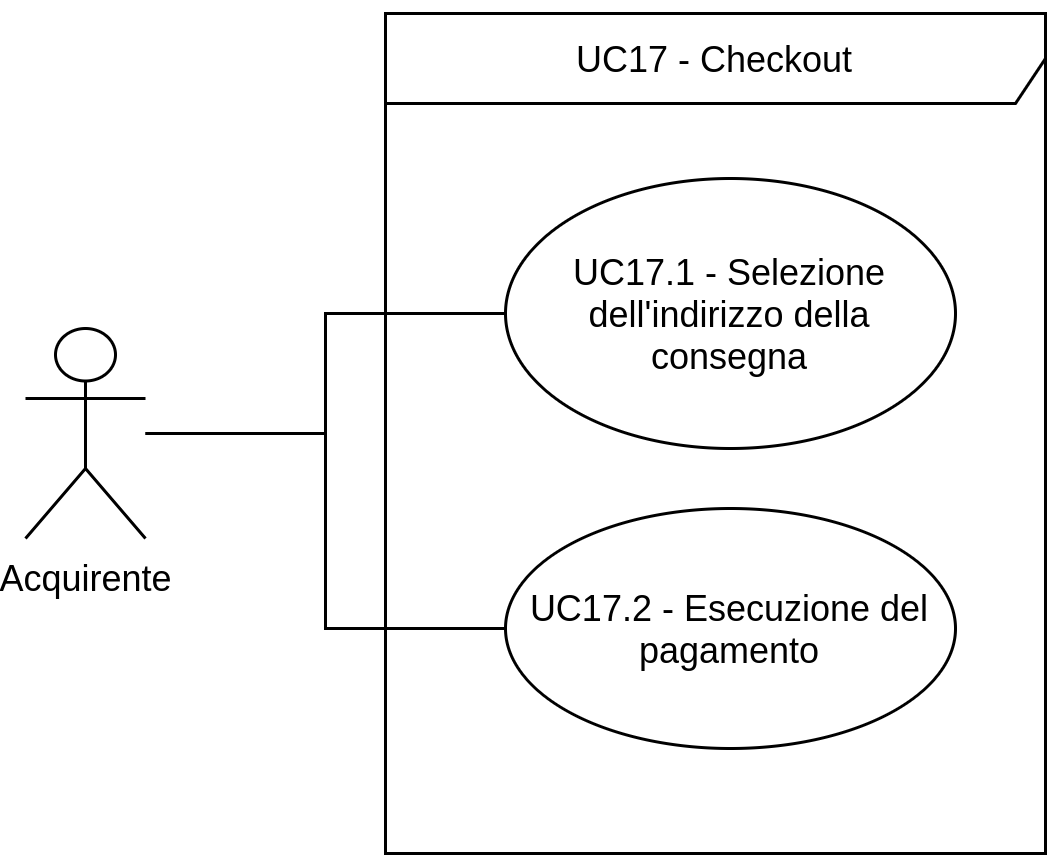
\includegraphics[scale=1]{Immagini/DiagrammiUC/Acquirente/Checkout.png}
    \caption{Diagramma di \actualUC: Checkout} 
    \label{fig:checkout}
\end{figure}

L'acquirente si trova nella schermata del carrello e vuole procedere al checkout per acquistare i prodotti scelti.
\begin{itemize}
    \item \textbf{Attori primari:} acquirente;
    \item \textbf{Attori secondari:} gestore dei pagamenti;
    \item \textbf{Precondizione:} l'acquirente si trova nella schermata del carrello e ha selezionato la funzione per il checkout;
    \item \textbf{Postcondizione:} l'acquirente ha terminato il checkout acquistando i prodotti nel carrello, il suo carrello risulterà vuoto e verrà reindirizzato alla schermata di riepilogo dell'ordine;
    \item \textbf{Scenario principale:} l'acquirente si trova nella schermata del carrello e seleziona la funzionalità per procedere con il checkout. In seguito eseguirà le seguenti azioni:
    \begin{itemize}
    	\item (UC\ref{checkout.indirizzo}) - Selezionare l'indirizzo di consegna;
    	\item Inserire possibili informazioni aggiuntive per la consegna dell'acquisto;
        \item (UC\ref{checkout.pagamento}) - Eseguire il pagamento.
    \end{itemize}
    Se il pagamento è andato a buon fine, verrà visualizzato un messaggio il quale segnalerà la buona riuscita del pagamento e verrà visualizzata la schermata di riepilogo dell'ordine;
    \item \textbf{Estensioni:}
    \begin{enumerate}[label=\lett]
        \item Se il pagamento fallisce per un errore del gestore dei pagamenti:
        \begin{itemize}
            \item (UC\ref{estensione:pagamento-fallito}) - Verrà visualizzato il messaggio di errore pagamento non andato a buon fine;
            \item Il carrello non verrà svuotato;
            \item L'acquirente verrà reindirizzato alla schermata del carrello.
        \end{itemize}
    \end{enumerate}
\end{itemize}

\subUC{Selezione dell'indirizzo della consegna}
\label{checkout.indirizzo}

L'acquirente seleziona l'indirizzo della consegna, ovvero dove verrà recapitato l'acquisto, tra gli indirizzi di consegna precedentemente inseriti.
\begin{itemize}
    \item \textbf{Attori primari:} acquirente;
    \item \textbf{Precondizione:} l'acquirente si trova nell'operazione di checkout;
    \item \textbf{Postcondizione:} l'acquirente ha selezionato l'indirizzo di consegna;
    \item \textbf{Scenario principale:} l'acquirente si trova nell'operazione di checkout e seleziona uno tra gli indirizzi di consegna precedentemente inseriti;
    \item \textbf{Scenari alternativi:}
    \begin{enumerate}[label=\lett]
        \item Se sono presenti altri indirizzi, l'acquirente ha eseguito almeno un ordine e non seleziona alcun indirizzo per la consegna, allora verrà utilizzato l'indirizzo a cui è stato recapitato l'ultimo ordine;
        \item Se non è presente alcun indirizzo da utilizzare per la consegna, allora verrà mostrato un messaggio il quale indicherà l'obbligo di dover inserire un indirizzo di consegna per poter proseguire con il checkout. In seguito l'indirizzo appena inserito verrà selezionato automaticamente per proseguire con la consegna.
    \end{enumerate}
\end{itemize}

\subUC{Esecuzione del pagamento}
\label{checkout.pagamento}

L'acquirente procede al pagamento attraverso il servizio fornito dal gestore dei pagamenti.
\begin{itemize}
    \item \textbf{Attori primari:} acquirente;
    \item \textbf{Attori secondari:} gestore dei pagamenti;
    \item \textbf{Precondizione:} l'acquirente è nell'operazione di checkout e ha selezionato l'indirizzo a cui consegnare l'ordine;
    \item \textbf{Postcondizione:} l'acquirente ha effettuato il pagamento;
    \item \textbf{Scenario principale:} l'acquirente è nell'operazione di checkout, ha selezionato l'indirizzo a cui consegnare l'ordine e seleziona la funzione di pagamento. A questo punto, il gestore dei pagamenti si occuperà di offrire all'acquirente tutto ciò di cui ha bisogno per ultimare l'ordine attraverso il pagamento.
\end{itemize}

%%%%%%%%%%%%%%%%%%%%%%%%%%%%%%%%%%%%%%%%%%%%%%%%%%%%%%%%%%%%%%%%%%%%%%%%%%%%%%%%%%%%%%%%%%%%%%%%%%%%%%%%%%%%%%%%%%%%%%%%%%%%%%%%%%%%%%%%%%%%%%%%%%%%%%%%%%%%%%%%%%%%%%%%%%%%%%